
\chapter{Introduzione}

\section{Motivazione}
% Spiegare il perché l'ho fatto Dati importanti, piccole e medie imprese devono sfruttare software opensource disponibili a tutti che permetto di passare da una frase experimental a production ready

Le piccole e medie imprese sono sempre più informatizzate e dipendenti da servizi informatici per poter svolgere il loro lavoro. Per questo motivo scoprire e analizzare il traffico anomalo in transito sulle reti aziendali è sempre più importante, il nostro obiettivo è farlo ad un basso costo, senza aggiungere hardware o applicativi che richiedano molta potenza di calcolo o di banda, sfruttando i router che compongono la rete. Punteremo a scoprire le anomalie nei dati di rete sui singoli flussi e nei dati aggregati analizzando alcune metriche su un server aggiuntivo che si occuperà anche di mitigare l'attacco informando i router sui flussi da bloccare o limitare.
Gli attacchi maggiormente presi in considerazione in questa tesi saranno gli attacchi di ``Distributed Denial of Service'', ma gli stessi principi potranno essere applicati anche ad altre tipologie di anomalie.
% problema delle botnets
Inoltre l'analisi dei dati raccolti sull'utilizzo della rete potrà portare anche alla risoluzioni di problemi di rete non derivanti da attacchi.

\section{Collaborazione con Tiesse s.p.a.}

Questa tesi è stata sviluppata in collaborazione con Tiesse s.p.a.: un'azienda che progetta e realizza, interamente in Italia, router e dispositivi M2M, con connettività wired e mobile.

L'azienda ha oltre 20 anni di esperienza, ed è stata riconosciuta come uno dei maggiori fornitori di CPE a banda larga e wireless su reti 3G/4G dalla maggior parte delle compagnie telefoniche. Oltre alla produzione e alla progettazione di router e apparecchiature di rete sviluppa progetti custom, sia hardware che software. I prodotti Tiesse sono particolarmente adatti ad applicazioni Business e Mission Critical per il Corporate Networking.

L'azienda è sempre attiva sull'aspetto di ricerca e sviluppo, anche tramite collaborazioni con il Politecnico di Torino e in particolare negli ultimi anni ha messo il focus su soluzioni software per la sicurezza e l'analisi dei dati di rete.

La sede centrale dell'azienda si trova ad Ivrea, ma possiede anche sedi distaccate a Torino, Avezzano e Roma.

% Scrivo quello dell'abstractafd
% lavoro svolto in collaborazione e in parte in presenza presso l'azienda spa di Ivrea

% Sezione in cui parlo di cui fa Tiesse spa
% - presento azienda
% - location e sedi distaccate
% - parlare della collaborazione con il poli => sempre in collaborazione per ricerca e sviluppo in particolare negli ultimi anni con un focus sugli aspetti di sicurezza e analisi dati di rete e non solo hw => prendere spunto anche dal sito
% - prendere ispirazione dalla slide tiesse di itasec

\section{Scenario}
\begin{figure}[]
    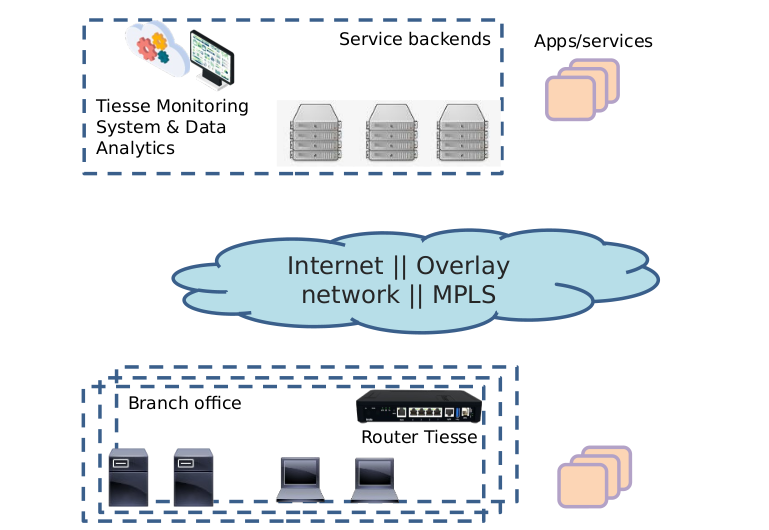
\includegraphics[width=\hsize]{images/introduzione/scenario_2.png}
    \caption{Scenario rete Tiesse e clienti}
    \label{fig:scenario_1}
    \centering    

\end{figure}

Nello sviluppo della nostra soluzione abbiamo preso in considerazione un tipico scenario aziendale, in cui esiste una sede centrale, ben protetta e su cui sono ospitati i servizi dell'azienda e tante sedi periferiche: uffici, negozi o altro, collegati ai servizi della sede centrale tramite un overlay MPLS o una VPN.
Le sedi periferiche sono quelle più esposte sotto l'aspetto della sicurezza, \uline{anche solo per il fatto che sono in numero maggiore, spesso non ci sono i responsabili dell'IT in sede e solitamente sono meno controllate rispetto la sede centrale}. Per questo motivo il nostro obiettivo è quello di proteggere i servizi, gli applicativi aziendali e la rete centrale dai dispositivi malevoli connessi alle reti degli uffici.
L'organizzazione di Tiesse e di molti suoi clienti è caratterizzata dallo scenario in figura ~\ref{fig:scenario_1}. Utilizzando questa struttura di rete per effettuare la raccolta, l'analisi del traffico e le prove, ci siamo basati su un esempio di sede periferica, nel nostro caso un ufficio dell'azienda situato a Torino, con l'obiettivo di proteggere i servizi aziendali presenti nella sede centrale di Ivrea a cui l'ufficio è collegato tramite una VPN.

Un altro caso possibile di utilizzo di questa soluzione è la distribuzione dei servizi in cloud, in cui l'azienda non ha il controllo dell'infrastruttura di rete e sfrutta i router thrusted nelle reti degli uffici per analizzare il traffico.


\begin{figure}[]
    \label{fig:scenario_2}
    %https://lucid.app/lucidchart/8119c7e9-e2e1-4dbb-b55f-bebf6c97af2d/edit?beaconFlowId=3612F8C43004D8D2&page=0_0#
    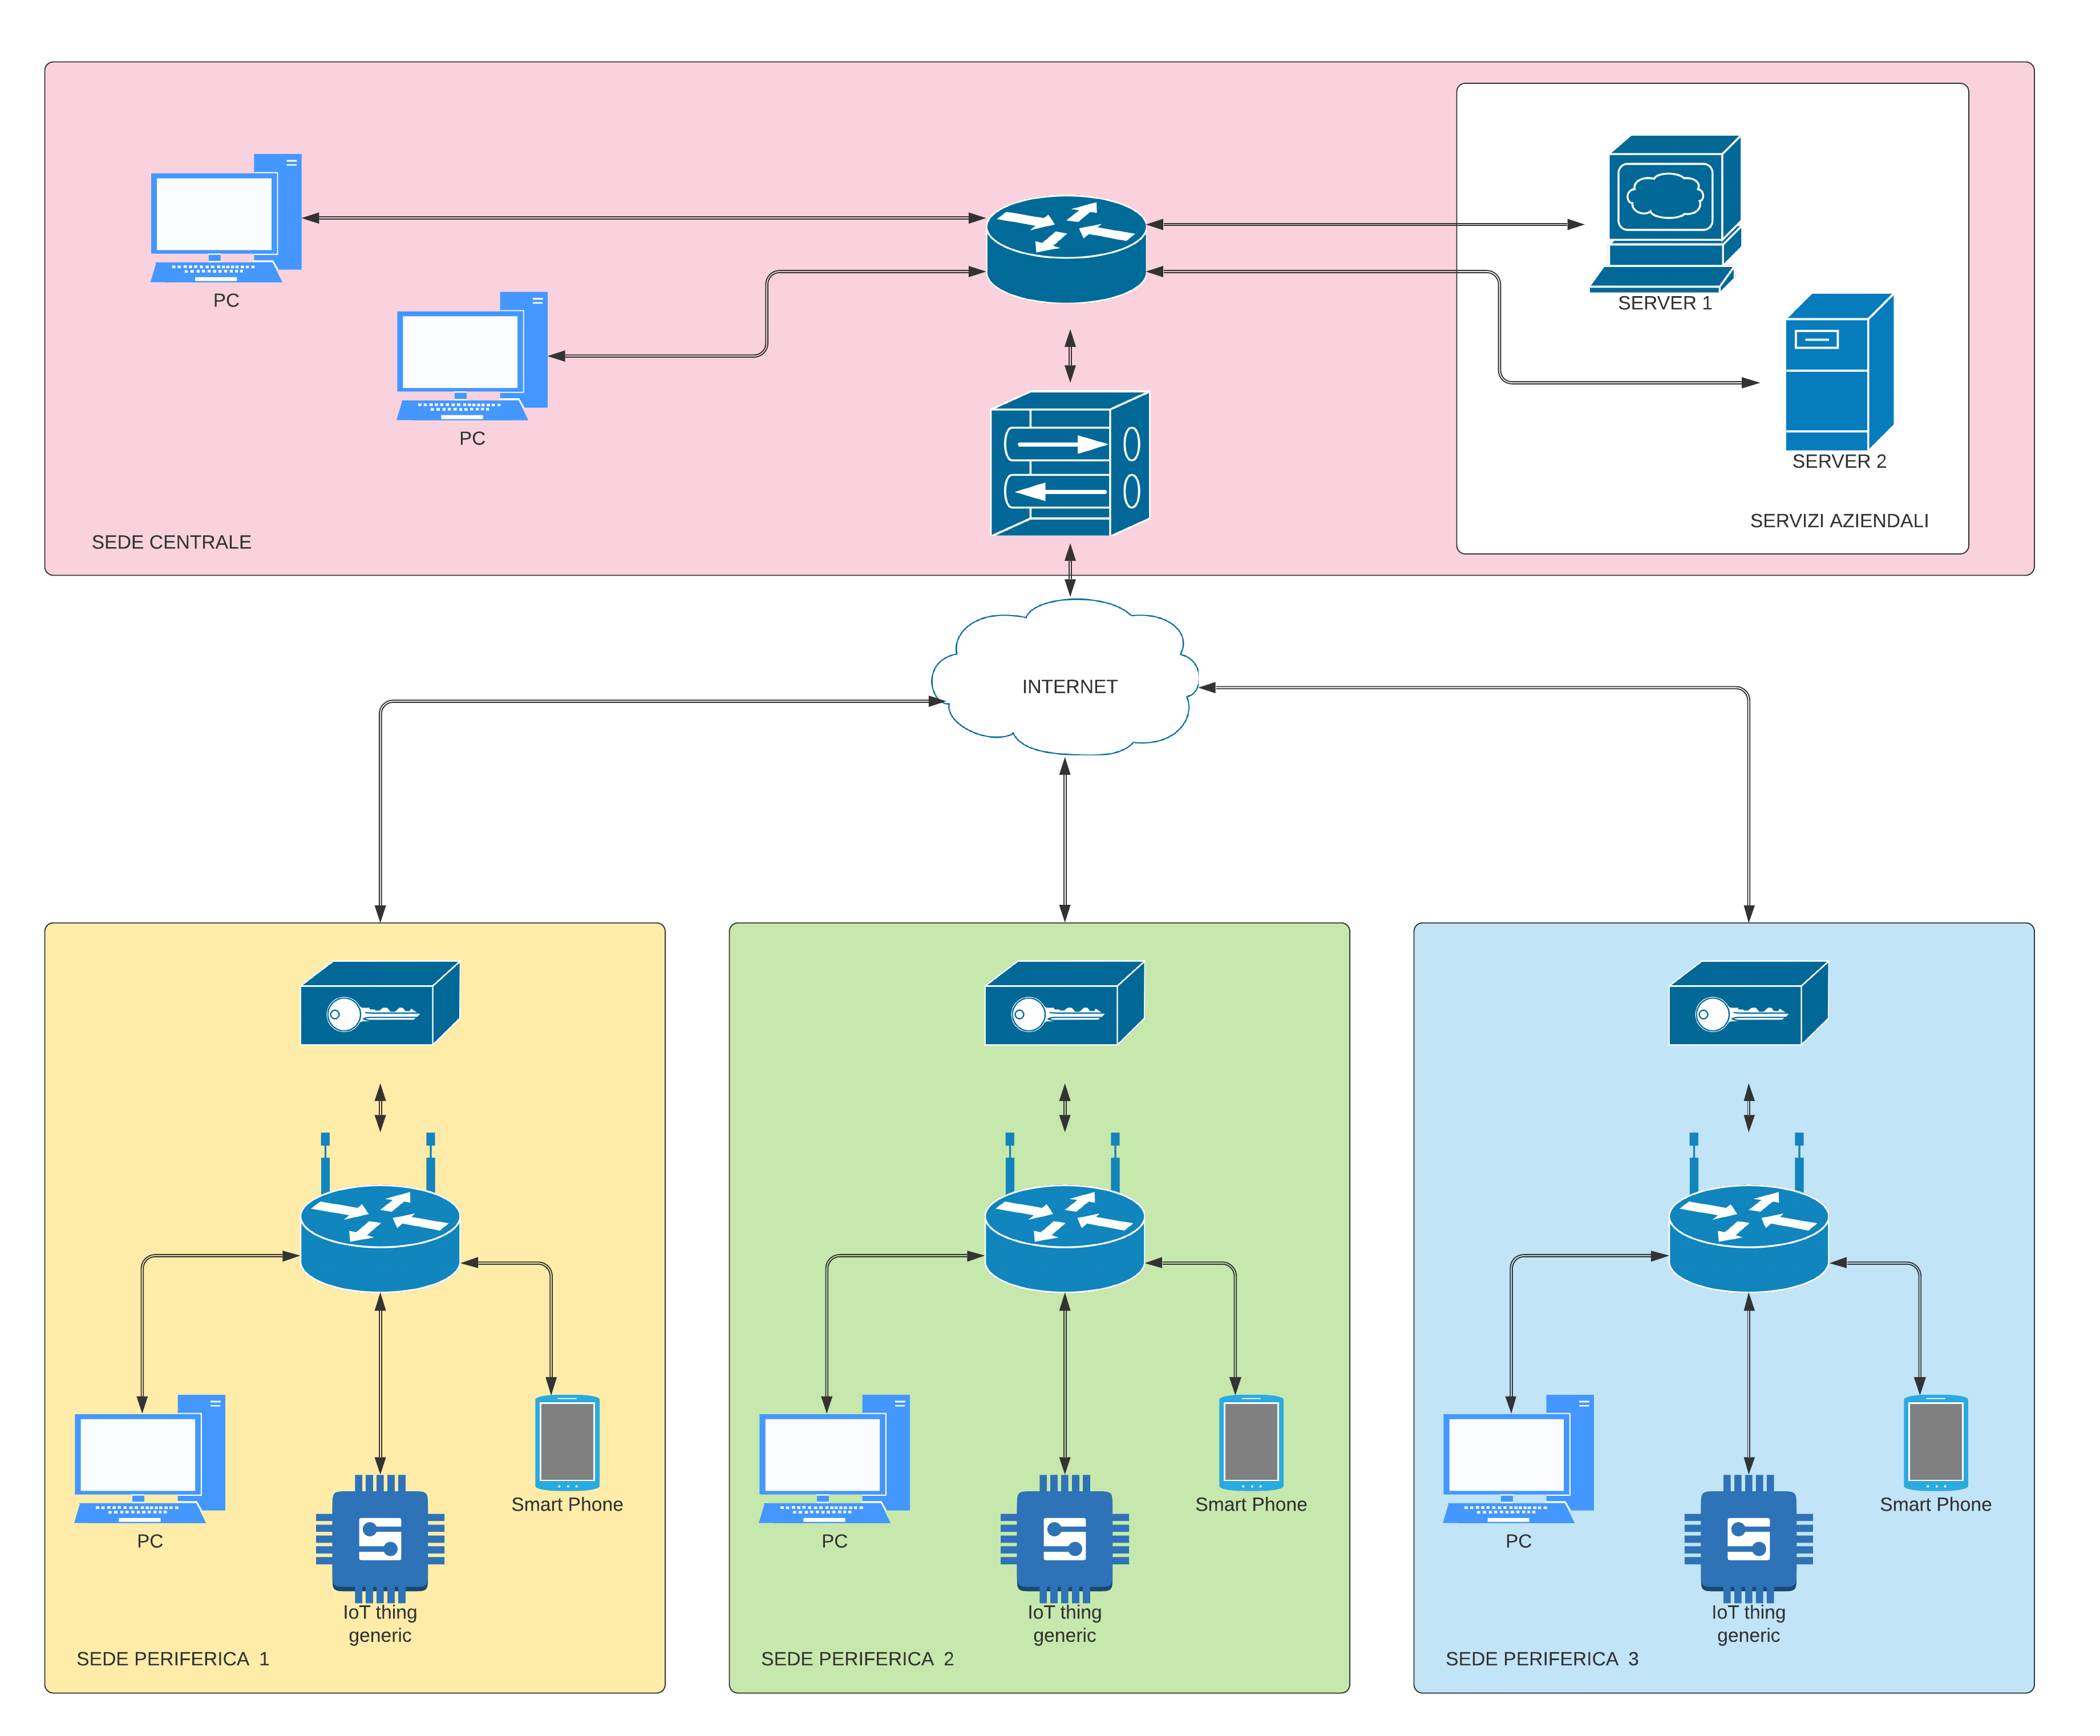
\includegraphics[width=\hsize]{images/introduzione/scenario.png}
    \caption{Scenario rete Tiesse e clienti}
    \centering
\end{figure}

\section{Riassunto}

Il nostro obiettivo è costruire un sistema di anomaly detection con struttura distribuita: nei router delle sedi periferiche dell'azienda vengono raccolte informazioni sul traffico e in un server posizionato nella sede centrale essi vengono analizzati, consentendogli di identificare da quale sede proviene il traffico anomalo. In base al risultato verranno prese decisioni sulle azioni da intraprendere. Questa architettura permette di sfruttare dispositivi già esistenti e non aggiunge molta complessità all'infrastruttura informatica aziendale. Utilizzando una soluzione distribuita è possibile bloccare gli attacchi e il traffico malevolo lontano dalla sede centrale, questo permette di essere più efficienti nel contrastare un attacco proveniente da una o più sedi periferiche, senza influenzare il comportamento di altre sedi.

La scelta del sistema di anomaly detection è ricaduta sull'utilizzo di una rete neurale basata su autoencoders a causa della loro semplicità d'uso, poiché non necessitano di dati etichettati per la fase di allenamento, quindi è facile ottenere grandi quantità di dati in qualsiasi contesto aziendale rendendo veloce l'introduzione di questo sistema, unita alla facilità di utilizzo delle API messe a disposizione da Keras e TensorFlow, le quali consentono di creare facilmente il modello e allenare la rete. Inoltre la precisione dei sistemi, utilizzanti autoencoders vanilla o varianti, è paragonabile ad altri sistemi a scapito, in alcuni casi, di un piccolo aumento di tempo in fase di test.

La scelta delle features da monitorare è una componente fondamentale per ottenere buoni risultati, nel nostro caso abbiamo usato dati molto aggregati per la prima fase di analisi, raccolti da collectd, nDPI e un nostro tool, i quali monitorano per esempio il throughput medio aggiornato ogni 10 secondi o il numero dei TCP syn in transito sul router nello stesso intervallo di tempo. La scelta della features è nata da un compromesso tra i dati necessari per rilevare al meglio le anomalie, la riduzione dei dati da salvare sul server e di conseguenza l'uso di banda usata per il trasferimento. Inoltre un problema che abbiamo dovuto tenere in considerazione è l'utilizzo di un acceleratore hardware nei router Tiesse, il quale permette un incremento della velocità di routing, ma rende difficile analizzare nel kernel i pacchetti senza perdita di prestazioni. I dati raccolti, sono successivamente mandati al server, nel nostro caso abbiamo usato un time series database (go-graphite) ed è possibile visualizzarli tramite Grafana, una dashboard open source per la visualizzazione di dati. Il nostro software per l’anomaly detection si interfaccia direttamente con il database per l’acquisizione e la scrittura dei dati. Ottenuti i dati e standardizzati, per un migliore funzionamento della rete neurale, vengono generate sequenze di lunghezza fissa per uniformare i dati di allenamento e valutazione da dare in input alla rete neurale.

L'utilizzo degli autoencoders permette di ottenere degli “anomaly score” per ogni sequenza di dati. Terminata la fase di allenamento della rete bisogna decidere sopra quali valori vogliamo considerare i dati anomali. Ipotizzato che tutti i dati forniti per il train siano regolari, le soglie sopra le quali dobbiamo considerare i dati anomali verranno prese dai massimi valori degli anomaly score per ogni feature. Anche la scelta del modello di rete è molto importante per ottenere un buon risultato nel rilevamento delle anomalie, per questo motivo abbiamo effettuato molte prove con diverse tipologie di reti: sia Dense feedforward, sia LSTM recurrent.

Mitigare gli attacchi DDoS è un problema di più difficile risoluzione rispetto alla sola rilevazione, bisogna conoscere maggiori informazioni sulla provenienza del flusso malevolo e il problema dei ``false positive'' è maggiormente sentito se ci prefiggiamo l'obiettivo di bloccare automaticamente i flussi malevoli, poichè dei falsi positivi significheranno un degrado della connessione di utenti legittimi.
Per la raccolta di maggiori informazioni riguardanti i flussi, in forma meno aggregata, abbiamo utilizzato un ulteriore tool in ascolto del traffico su un interfaccia, il software è stato sviluppato grazie all’utilizzo di eBPF (extended Berkeley Packet Filter), che permette il filtraggio e l'analisi dei pacchetti in transito in maniera molto efficiente utilizzando l’hook XDP (eXpress Data Path), un punto di aggancio ad alte prestazioni che permette di eseguire un programma eBPF nel primo punto possibile,  prima che qualsiasi altra manipolazione del pacchetto  possa avvenire.
Sul server di monitoraggio quando viene rilevata un'anomalia è possibile risalire su quale router sono transitati i dati sospetti, quindi viene notificato il router della sede periferica responsabile e viene messa in atto la fase di mitigazione. Questa fase raccogliendo dati in forma meno aggregata, è potenzialmente più dispendiosa in termini di risorse, per questo motivo la eseguiamo solo in presenza di un'anomalia sui dati aggregati.
Per metterla in atto per prima cosa dobbiamo raccogliere i dati sui flussi tramite eBPF, successivamente nella fase di decisione un software di anomaly detection strutturato in maniera simile al precedente o un amministratore di sistema decidono cos'è anomalo e infine sempre tramite eBPF blocchiamo o limitiamo il traffico proveniente da uno o più indirizzi IP.

Un altro accorgimento per limitare gli attacchi si basa sul limitare l’ip spoofing, tecnica sfruttata da molti attacchi DDoS. Nello scenario da noi ipotizzato il meccanismo di mitigazione è installato negli edge router delle sedi aziendali periferiche, in questa posizione possiamo ipotizzare che tutti i pacchetti in transito dalla sottorete del distaccamento, verso la sottorete della sede centrale o verso internet, siano stati generati da un host di quella sotto rete. Per questo motivo una soluzione per limitare il problema è impedire al router di effettuare l'inoltro di tutti i pacchetti provenienti da altre sottoreti tramite una regola iptables.


\section{Organizzazione della tesi}

La tesi nei successivi capitoli tratterà lo stato dell'arte dei sistemi anti-ddos esistenti (capitolo 2), mostrando come è possibile riconoscere un attacco e dove è meglio farlo per poterlo mitigare al meglio. Nel capitolo 3 approfondirà maggiormente lo stato dell'arte dei sistemi di anomaly detection da utilizzare per rilevare un attacco DDoS.
Nei capitoli 4 e 5 verrà illustrata la soluzione da noi proposta, focalizzandosi nel quarto sulla tecnica per rilevare un'anomalia e nel quinto su come mitigarla.
Nel capitolo 6 vengono menzionati possibili lavori futuri e nel 7 le conclusioni con delle considerazioni sulla soluzione proposta.